\documentclass{beamer}
\usepackage{hyperref}
\usepackage{parskip}
\usepackage{verbatim}
\usepackage{tabularx}
\usepackage{amsmath}
\usepackage{comment}

% \usetheme{Madrid}
\usetheme{Boadilla}
% \usetheme{Montpellier}
\usepackage{Sweave}
\begin{document}
\Sconcordance{concordance:Lecture_2.2.tex:Lecture_2.2.Rnw:%
1 11 1 1 0 1416 1}


\title{BIOS 545 Week 3, Lecture 2}
\author{Steve Pittard wsp@emory.edu}
\subtitle{Department of Biostatistics and Bioinformatics}
\date{\today}

\maketitle


%% Data Frames continued
\section{Data Frames}


\begin{frame}[fragile]
\frametitle{Data Frames - Merge}
\begin{itemize}

\item Merging data frames is possible  

\item But we don't often encounter two or more similar
enough data frames that we can merge them easily. 

\item Usually we pick and choose columns from a number of data frames to build a new data frame. 

\item But this isn't easy either since not all observations are from the same population.

\item Always work with the \emph{minimum} amount of data necessary for a given analysis 

\item There is no reason to create a big data frame if you are only going to be using 20 percent of 
the attributes/columns.
\end{itemize}
\end{frame}



\begin{frame}[fragile]
\frametitle{Data Frames - Merge}
Merging data frames is possible. You have to select a ``key'' that is common to both data frames to make this work. Pick a column(s) that links the two data frames
\footnotesize
\begin{verbatim}
df1 <- data.frame(indiv_id = 1:4, snp1 = c(1,1,0,1), snp2 = c(1,1,0,0)) 

df2 <- data.frame(indiv_id = c(1,3,4,6), cov1 = c(1.14,4.50,0.80,1.39), 
                                          cov2 = c(74.6,79.4,48.2,68.1))

df1
  indiv_id snp1 snp2
        1    1    1
        2    1    1
        3    0    0
        4    1    0
df2
  indiv_id cov1 cov2
        1 1.14 74.6
        3 4.50 79.4
        4 0.80 48.2
        6 1.39 68.1

merge(df1, df2, by="indiv_id", all=TRUE)
  indiv_id SNP1 SNP2 cov1 cov2
        1    1    1 1.14 74.6
        2    1    1   NA   NA
        3    0    0 4.50 79.4
        4    1    0 0.80 48.2
        6   NA   NA 1.39 68.1
\end{verbatim}
\end{frame}


\begin{frame}[fragile]
\frametitle{Data Frames - Merge}
The ``indiv\_id'' column looks like it will do the trick
\footnotesize
\begin{verbatim}
df1
  indiv_id snp1 snp2
        1    1    1
        2    1    1
        3    0    0
        4    1    0
df2
  indiv_id cov1 cov2
        1 1.14 74.6
        3 4.50 79.4
        4 0.80 48.2
        6 1.39 68.1

merge(df1, df2, by="indiv_id", all=TRUE)
  indiv_id SNP1 SNP2 cov1 cov2
        1    1    1 1.14 74.6
        2    1    1   NA   NA
        3    0    0 4.50 79.4
        4    1    0 0.80 48.2
        6   NA   NA 1.39 68.1
\end{verbatim}
\end{frame}


\begin{frame}[fragile]
\frametitle{Data Frames - Merge}
Pay attention to the ``all.x'' and ``all.y'' arguments as it helps you specify which records you want to the include 
\footnotesize
\begin{verbatim}
df1
  indiv_id snp1 snp2
        1    1    1
        2    1    1
        3    0    0
        4    1    0
df2
  indiv_id cov1 cov2
        1 1.14 74.6
        3 4.50 79.4
        4 0.80 48.2
        6 1.39 68.1

merge(df1, df2, by="indiv_id", all.y=T)
  indiv_id snp1 snp2 cov1 cov2
1        1    1    1 1.14 74.6
2        3    0    0 4.50 79.4
3        4    1    0 0.80 48.2
4        6   NA   NA 1.39 68.1
\end{verbatim}
\end{frame}

\begin{frame}[fragile]
\frametitle{Data Frames - Merge}
Note that the merge columns do not have to be named the same thing in each data frame as long as they refer to the same thing
\footnotesize
\begin{verbatim}
names(df2) <- c("id","cov1","cov2")

head(df1,2)
  indiv_id snp1 snp2
1        1    1    1
2        2    1    1

head(df2,2) 
  id cov1 cov2
1  1 1.14 74.6
2  3 4.50 79.4

merge(df1,df2,by.x="indiv_id",by.y="id",all=TRUE)
  indiv_id snp1 snp2 cov1 cov2
1        1    1    1 1.14 74.6
2        2    1    1   NA   NA
3        3    0    0 4.50 79.4
4        4    1    0 0.80 48.2
5        6   NA   NA 1.39 68.1
\end{verbatim}
\end{frame}

\begin{frame}[fragile]
\frametitle{Data Frames - split}
\begin{itemize}
\item The split function lets us break up a data frame based on a grouping variable
\item Let's say we want to split up mtcars based on the number of cylinders which take on the values 4,6,8
\item Use the split command which gives back a list with each element containing a part of the data frame corresponding to each cylinder group
\item Without using split you could do:
\end{itemize}
\footnotesize
\begin{verbatim}
eight.cyl <- mtcars[mtcars$cyl == 8,]

six.cyl <- mtcars[mtcars$cyl == 6, ]

four.cyl <- mtcars[mtcars$cyl == 4, ]
\end{verbatim}
\end{frame}

%

\begin{frame}[fragile]
\frametitle{Data Frames - split}
But what if we had 10 categories we wanted to split by ? The \textbf{split} function does scale well so use it !
\footnotesize
\begin{verbatim}
hold <- split(mtcars, mtcars$cyl) 

str(hold,max.level=1)
List of 3
 $ 4:'data.frame':  11 obs. of  11 variables:
 $ 6:'data.frame':	7 obs. of  11 variables:
 $ 8:'data.frame':	14 obs. of  11 variables:

head(hold[[1]],3) # Show the first 3 lines of the first list element 

            mpg cyl  disp hp drat   wt  qsec vs am gear carb
Datsun 710 22.8   4 108.0 93 3.85 2.32 18.61  1  1    4    1
Merc 240D  24.4   4 146.7 62 3.69 3.19 20.00  1  0    4    2
Merc 230   22.8   4 140.8 95 3.92 3.15 22.90  1  0    4    2
\end{verbatim}
\end{frame}

%

\begin{frame}[fragile]
\frametitle{Data Frames - split}
Why is this useful ? Well we might want to focus in on only the cars occupying a certain cylinder group while ignoring the rest. So if we wanted only the 8 cylinder cars:
\footnotesize
\begin{verbatim}
hold <- split(mtcars, mtcars$cyl) 

sapply(hold,nrow)
 4  6  8 
11  7 14 

eight.cyl <- hold$`8`   

# -OR-

eight.cyl <- hold[[3]]

\end{verbatim}
\end{frame}
%
\begin{frame}[fragile]
\frametitle{Data Frames - split}
Because what we get back is a list we can use lapply to look at the first few records of each element which is a data frame
\footnotesize
\begin{verbatim}
hold <- split(mtcars, mtcars$cyl) 

str(hold,max.level=1)
List of 3
 $ 4:'data.frame':  11 obs. of  11 variables:
 $ 6:'data.frame':  7 obs. of  11 variables:
 $ 8:'data.frame':	14 obs. of  11 variables:
\end{verbatim}
\end{frame}


\begin{frame}[fragile]
\frametitle{Data Frames - split}
\footnotesize
\begin{verbatim}
lapply(hold,head,3)
$`4`
            mpg cyl  disp hp drat   wt  qsec vs am gear carb
Datsun 710 22.8   4 108.0 93 3.85 2.32 18.61  1  1    4    1
Merc 240D  24.4   4 146.7 62 3.69 3.19 20.00  1  0    4    2
Merc 230   22.8   4 140.8 95 3.92 3.15 22.90  1  0    4    2

$`6`
                mpg cyl disp  hp drat    wt  qsec vs am gear carb
Mazda RX4      21.0   6  160 110 3.90 2.620 16.46  0  1    4    4
Mazda RX4 Wag  21.0   6  160 110 3.90 2.875 17.02  0  1    4    4
Hornet 4 Drive 21.4   6  258 110 3.08 3.215 19.44  1  0    3    1

$`8`
                   mpg cyl  disp  hp drat   wt  qsec vs am gear carb
Hornet Sportabout 18.7   8 360.0 175 3.15 3.44 17.02  0  0    3    2
Duster 360        14.3   8 360.0 245 3.21 3.57 15.84  0  0    3    4
Merc 450SE        16.4   8 275.8 180 3.07 4.07 17.40  0  0    3    3
\end{verbatim}
\end{frame}


\begin{frame}[fragile]
\frametitle{Data Frames - split}
We could write our own summary function. While it is an advanced idea at this point, it is good for you too see this kind of approach as it is common in R. This example gives the mean MPG for each cylinder group:
\small
\begin{verbatim}
# We create our own function and apply it to each element of "hold"

hold <- split(mtcars,mtcars$cyl) 
sapply(hold, function(x) mean(x$mpg))

   4        6        8 
26.66364 19.74286 15.10000 
\end{verbatim}
\end{frame}

%



\begin{frame}[fragile]
\frametitle{Data Frames - order/sort}
Let's take a look at what the order command does. It returns the record/row  numbers of the data frame from lowest MPG to highest. So record \#15 must be the lowest MPG automobile in the set. And record \#20 must have the highest MPG
\footnotesize
\begin{verbatim}
order(mtcars$mpg)
 [1] 15 16 24  7 17 31 14 23 22 29 12 13 11  6  5 10 25 30  
[19]  1  2  4 32 21  3  9 8 27 26 19 28 18 20

mtcars[15,]
                    mpg cyl disp  hp drat   wt  qsec vs am gear carb
Cadillac Fleetwood 10.4   8  472 205 2.93 5.25 17.98  0  0    3    4

mtcars[20,]
                mpg cyl disp hp drat    wt qsec vs am gear carb
Toyota Corolla 33.9   4 71.1 65 4.22 1.835 19.9  1  1    4    1
\end{verbatim}
\end{frame}

%


\begin{frame}[fragile]
\frametitle{Data Frames - order/sort}
Ordering and sorting data frames is an important technique 
\footnotesize
\begin{verbatim}
# sort by mpg (ascending)
newdata <- mtcars[order(mtcars$mpg),] 

                     mpg cyl  disp  hp drat    wt  qsec vs am gear carb
Cadillac Fleetwood  10.4   8 472.0 205 2.93 5.250 17.98  0  0    3    4
Lincoln Continental 10.4   8 460.0 215 3.00 5.424 17.82  0  0    3    4
Camaro Z28          13.3   8 350.0 245 3.73 3.840 15.41  0  0    3    4
Duster 360          14.3   8 360.0 245 3.21 3.570 15.84  0  0    3    4

newdata <- mtcars[rev(order(mtcars$mpg)),]  

                     mpg cyl  disp  hp drat    wt  qsec vs am gear carb
Toyota Corolla      33.9   4  71.1  65 4.22 1.835 19.90  1  1    4    1
Fiat 128            32.4   4  78.7  66 4.08 2.200 19.47  1  1    4    1
Honda Civic         30.4   4  75.7  52 4.93 1.615 18.52  1  1    4    2
Lotus Europa        30.4   4  95.1 113 3.77 1.513 16.90  1  1    5    2
\end{verbatim}
\end{frame}

\begin{frame}[fragile]
\frametitle{Data Frames - order/sort}
Ordering and sorting data frames is an important technique 
\footnotesize
\begin{verbatim}
newdata <- mtcars[order(-mtcars$mpg),]

head(newdata)
                mpg cyl  disp  hp drat    wt  qsec vs am gear carb
Toyota Corolla 33.9   4  71.1  65 4.22 1.835 19.90  1  1    4    1
Fiat 128       32.4   4  78.7  66 4.08 2.200 19.47  1  1    4    1
Honda Civic    30.4   4  75.7  52 4.93 1.615 18.52  1  1    4    2
Lotus Europa   30.4   4  95.1 113 3.77 1.513 16.90  1  1    5    2

\end{verbatim}
\end{frame}

\begin{frame}[fragile]
\frametitle{Data Frames - sample}
The \textbf{sample()} function is quite useful when you want to take, well, a sample of your data. You can sample with or without replacement. The basic function works as follows: 
\footnotesize
\begin{verbatim}
# Create a vector of numbers from 1 to 20
my_vec <- 1:20

sample(my_vec,10,replace=TRUE)    # Repetition is possible
 [1]  3 20 16 14 16 10 18  7  7  6

sample(my_vec, 10, replace=TRUE)  # Different results each time
 [1]  5  1  2  2 19  8 20 11  3 19

sample(my_vec, 10, replace=FALSE) # Don't replace sampled numbers
 [1]  2  8  9  6 17 18  3  5 14 15

sample(1:20, 10, replace=FALSE)   # Short cut
 [1] 13  6  4 14  3 19 16 17 20 12

\end{verbatim}
\end{frame}

\begin{frame}[fragile]
\frametitle{Data Frames - sample}
But how do you sample from a data frame ? We want a random sample of 10 records from mtcars 
\footnotesize
\begin{verbatim}
my_records <- sample(1:nrow(mtcars), 10, replace = FALSE)

my_records
 [1] 21  6  9 30 29 28  3 11 12  1

sample_of_ten <- mtcars[my_records,]

                mpg cyl  disp  hp drat    wt  qsec vs am gear carb 
Toyota Corona  21.5   4 120.1  97 3.70 2.465 20.01  1  0    3    1      
Valiant        18.1   6 225.0 105 2.76 3.460 20.22  1  0    3    1      
Merc 230       22.8   4 140.8  95 3.92 3.150 22.90  1  0    4    2      
Ferrari Dino   19.7   6 145.0 175 3.62 2.770 15.50  0  1    5    6      
Ford Pantera L 15.8   8 351.0 264 4.22 3.170 14.50  0  1    5    4      
Lotus Europa   30.4   4  95.1 113 3.77 1.513 16.90  1  1    5    2      
Datsun 710     22.8   4 108.0  93 3.85 2.320 18.61  1  1    4    1      
Merc 280C      17.8   6 167.6 123 3.92 3.440 18.90  1  0    4    4      
Merc 450SE     16.4   8 275.8 180 3.07 4.070 17.40  0  0    3    3      
Mazda RX4      21.0   6 160.0 110 3.90 2.620 16.46  0  1    4    4      

\end{verbatim}
\end{frame}

%% Section Programming Stuctures

\section{Programming Stuctures}

\begin{frame}[fragile]
\frametitle{Programming Structures}
\begin{center}
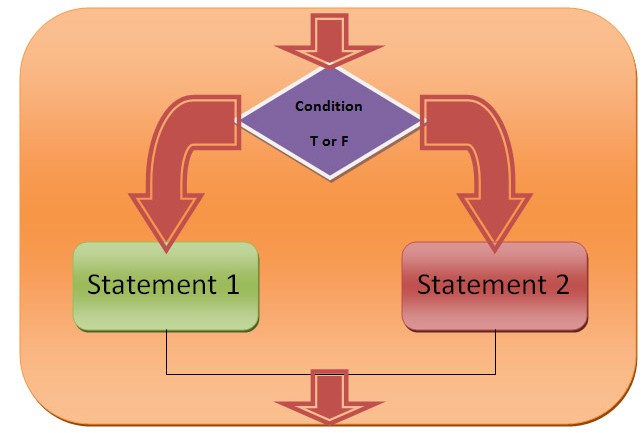
\includegraphics{../IMG/control.png}
\end{center}
\end{frame}


\begin{frame}[fragile]
\frametitle{Programming Structures}
Goals for this Session:
\begin{itemize}
\item Understand the for-loop structure and how to use it 

\item "Walk" through a vector while accumulating a sum, computing a product, or some other operation.

\item "Walk" though a matrix by row, (or column), while accumulating a sum, computing a product or some other arithmetic operation.

\item "Walk" through a data frame by row to compute something. Also process the results of a previous "split" operation.

\item Understand the if statement and how to branch based on the value of a vector or matrix element. 

\item Also use the if statement in conjunction with the for loop to do some processing.

\end{itemize}
\end{frame}

%

\begin{frame}[fragile]
\frametitle{Programming Structures}
Some things to keep in mind for getting better with programming structures
\begin{itemize}
\item Put the statements in the Editor window of RStudio and perfect them there. You can highlight sections of code and hit the "run" button

\item You will most definitely make mistakes when writing loops. It is guaranteed. 
Better to get familiar with the most common mistakes ahead of time

\item Work through the labs ! 

\item The next assignment will assume facility with these structures
\end{itemize}
\end{frame}

%

\begin{frame}[fragile]
\begin{center}
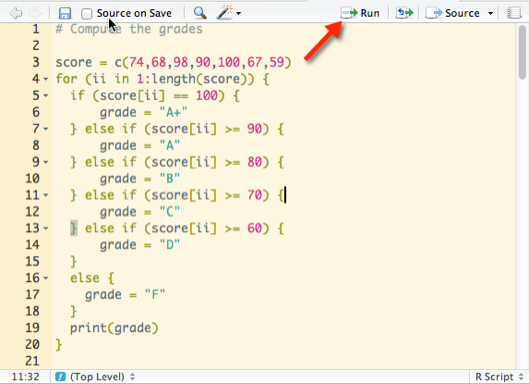
\includegraphics{../IMG/rstudioedit.png}
\end{center}
\end{frame}

%

\begin{frame}[fragile]
Go to Preferences -> Code Editing to turn on ``insert matching parens/braces'' 
\begin{center}
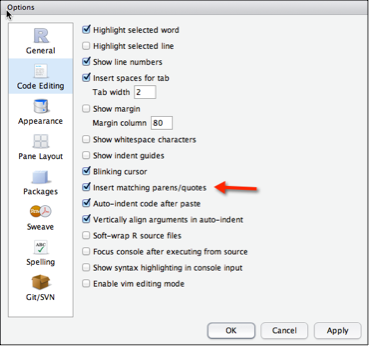
\includegraphics{../IMG/braces.png}
\end{center}
\end{frame}

%
\subsection{for loop}
\begin{frame}[fragile]
\frametitle{Programming Structures - for }
This is a looping construct that let's you do some things for a specific number of times.
\newline
\\
``name'' is some index variable that takes on values returned by ``expr\_1'', which is almost always some type of sequence. It could represent the length of a vector or a row of a matrix.

\small
\begin{verbatim}
for (name in expr_1) {
   expr_2
}

for (ii in 1:3) {
  print(ii)
}

[1] 1
[1] 2
[1] 3

\end{verbatim}
\end{frame}

%

\begin{frame}[fragile]
\frametitle{Programming Structures - for }
Better to generalize this - use the \textbf{length()} function so the loop will work with a vector of any size
\footnotesize
\begin{verbatim}
x <- rnorm(3)
for (ii in 1:length(x)) {
  print(ii)
}

[1] 1
[1] 2
[1] 3

# Here we access the actual values of x

x <- rnorm(3)
for (ii in 1:length(x)) {    
   print(x[ii])
}
[1] -0.6257547
[1] 0.39524
[1] -1.955594
\end{verbatim}
\end{frame}

%

\begin{frame}[fragile]
\frametitle{Programming Structures - for }
Consider the example wherein we have a x values that we want to provide as input into some function that will generate y values. 
\footnotesize
\begin{verbatim}
y <- vector()  # A blank vector
x <- 1:6
for (ii in 1:length(x)) {
  y[ii] <- x[ii]^2
}

x
[1] 1 2 3 4 5 6
y
[1]  1  4  9 16 25 36
plot(x,y,main="Super Cool Data Plot",type="b",pch=19,col="red")

\end{verbatim}
\end{frame}

%

\begin{frame}[fragile]
\frametitle{Programming Structures - for }
\begin{center}
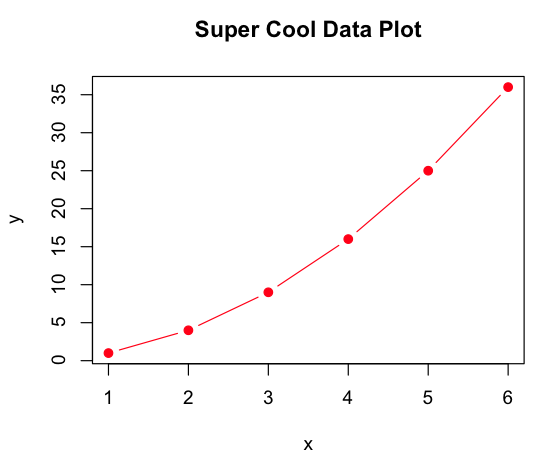
\includegraphics{../IMG/parab.png}
\end{center}
\end{frame}


%

\begin{frame}[fragile]
\frametitle{Programming Structures - for }
Here we use a for-loop to add up the elements in a vector and find the average. There are already functions in R to do this but knowing how to do it yourself is important
\footnotesize
\begin{verbatim}
x <-rnorm(1000,20,4)  # 1,000 random elements from a N(20,4)

mysum <- 0
for (ii in 1:length(x)) {
  mysum <- mysum + x[ii]
}
avg <- mysum / length(x)
cat("The average of this vector is:",avg,"\n")

[1] "The average of this vector is: 20.1320691898645"

We could clean up the output a little bit

cat("The average of this vector is:",round(avg,2),"\n")
[1] "The average of this vector is: 20.13"

\end{verbatim}
\end{frame}

%

\begin{frame}[fragile]
\frametitle{Programming Structures - for }
Given a vector find the smallest value without using the "min" function:
\footnotesize
\begin{verbatim}
set.seed(188)
x <- rnorm(1000)  # 1,000 random elements from a N(20,4)

# Set the min to the first element of x. Unless we are very lucky then 
# this will change as we walk through the vector

mymin <- x[1] 
for (ii in 1:length(x)) {
  if (x[ii] < mymin) {
     mymin <- x[ii]
  }
}

mymin
[1] -3.422185
 
min(mymin)       # The internal R function matches what we got
[1] -3.422185

\end{verbatim}
\end{frame}

%

\begin{frame}[fragile]
\frametitle{Programming Structures - for }
We can loop through data frames also. Let's see if we can compute the mean of the MPG for all cars. Note that we use the \textbf{nrow} function to get the number of rows to loop over 
\footnotesize
\begin{verbatim}
mpgsum <- 0
for (ii in 1:nrow(mtcars)) {
  mpgsum <- mpgsum + mtcars[ii,"mpg"]
}

mpgmean <- mpgsum/nrow(mtcars)   # Divide the sum by the # of records

cat("Mean MPG for all cars is:",mpgmean,"\n")
Mean MPG for all cars is: 20.09062 

mean(mtcars$mpg)
[1] 20.09062

\end{verbatim}
\end{frame}

%

\begin{frame}[fragile]
\frametitle{Programming Structures - for }
Remember the split command ? We can work with the output of that also. Relative to mtcars we let's split up the data frame by cylinder number, which is (4,6, or 8)
\footnotesize
\begin{verbatim}
mysplits <- split(mtcars, mtcars$cyl)

str(mysplits, max.level=1)
List of 3
 $ 4:'data.frame':  11 obs. of  11 variables:
 $ 6:'data.frame':	7 obs. of  11 variables:
 $ 8:'data.frame':	14 obs. of  11 variables:
\end{verbatim}
\normalsize
We get back a list that contains 3 elements each of which has a data frame corresponding to the number of cylinders. We could summarize each of these data frame elements using a for loop
\end{frame}


%

\begin{frame}[fragile]
\frametitle{Programming Structures - for }
\scriptsize
\begin{verbatim}
mysplits
$`4`
               mpg cyl  disp hp drat    wt  qsec vs am gear carb
Merc 240D     24.4   4 146.7 62 3.69 3.190 20.00  1  0    4    2
Merc 230      22.8   4 140.8 95 3.92 3.150 22.90  1  0    4    2
Toyota Corona 21.5   4 120.1 97 3.70 2.465 20.01  1  0    3    1
..
..

$`6`
                mpg cyl  disp  hp drat    wt  qsec vs am gear carb
Hornet 4 Drive 21.4   6 258.0 110 3.08 3.215 19.44  1  0    3    1
Valiant        18.1   6 225.0 105 2.76 3.460 20.22  1  0    3    1
Merc 280       19.2   6 167.6 123 3.92 3.440 18.30  1  0    4    4
Merc 280C      17.8   6 167.6 123 3.92 3.440 18.90  1  0    4    4
..
..

$`8`
                     mpg cyl  disp  hp drat    wt  qsec vs am gear carb
Hornet Sportabout   18.7   8 360.0 175 3.15 3.440 17.02  0  0    3    2
Duster 360          14.3   8 360.0 245 3.21 3.570 15.84  0  0    3    4
Merc 450SE          16.4   8 275.8 180 3.07 4.070 17.40  0  0    3    3
Merc 450SL          17.3   8 275.8 180 3.07 3.730 17.60  0  0    3    3
..
..
\end{verbatim}
\end{frame}


%

\begin{frame}[fragile]
\frametitle{Programming Structures - for }
\small
\begin{verbatim}
mysplit <- split(mtcars,mtcars$cyl)

for (ii in 1:length(mysplit)) {
   print(nrow(mysplit[[ii]]))
}

[1] 11
[1] 7
[1] 14

# This is equivalent to

sapply(mysplit, nrow)
 4  6  8 
11  7 14 
\end{verbatim}
\end{frame}

%

\begin{frame}[fragile]
\frametitle{Programming Structures - for }
\footnotesize
\begin{verbatim}
mysplit <- split(mtcars,mtcars$cyl)

for (ii in 1:length(mysplit)) {
   splitname <- names(mysplit[ii])
   cat("mean for",splitname,"cylinders is",mean(mysplit[[ii]]$mpg),"\n")
}
mean for 4 cylinders is 26.66364 
mean for 6 cylinders is 19.74286 
mean for 8 cylinders is 15.1 

# This is basically equivalent to 

sapply(mysplit, function(x) mean(x$mpg))
       4        6        8 
26.66364 19.74286 15.10000 
\end{verbatim}
\end{frame}

%

\begin{frame}[fragile]
\frametitle{Programming Structures - for }
What about looping over each split and pulling out only those cars with an manual transmission ? (am == 1) 
\footnotesize
\begin{verbatim}
data(mtcars)

mysplit <- split(mtcars,mtcars$cyl)

mylist <- list() # Setup a blank list to contain the subset results

for (ii in 1:length(mysplit)) {
  mylist[[ii]] <- subset(mysplit[[ii]], am == 1)
}

mylist

# Equivalent to:

lapply(mysplit, subset, am == 1)

\end{verbatim}
\end{frame}

%

%\begin{frame}[fragile]
%\frametitle{Programming Structures - for }
%What about looping over each split and sampling two records from each group ? 
%\footnotesize
%\begin{verbatim}
%for (ii in 1:length(mysplits)) {
%    recs <- sample(1:nrow(mysplits[[ii]]),2,F)
%    print(mysplits[[ii]][recs,])
%}
%             mpg cyl disp hp drat    wt  qsec vs am gear carb
%Honda Civic 30.4   4 75.7 52 4.93 1.615 18.52  1  1    4    2
%Fiat 128    32.4   4 78.7 66 4.08 2.200 19.47  1  1    4    1
%
%              mpg cyl disp  hp drat    wt  qsec vs am gear carb
%Mazda RX4 Wag  21   6  160 110  3.9 2.875 17.02  0  1    4    4
%Mazda RX4      21   6  160 110  3.9 2.620 16.46  0  1    4    4
%
%                     mpg cyl  disp  hp drat    wt  qsec vs am gear carb
%Merc 450SL          17.3   8 275.8 180 3.07 3.730 17.60  0  0    3    3
%Lincoln Continental 10.4   8 460.0 215 3.00 5.424 17.82  0  0    3    4
%
%\end{verbatim}
%\end{frame}


%

%\begin{frame}[fragile]
%\frametitle{Programming Structures - for }
%What about looping over each split and sampling two records from each group ?
%\footnotesize
%\begin{verbatim}
%lapply(mysplit, function(x) {
%                      recs = sample(1:nrow(x),2,F)
%                      return(x[recs,])
%                  })
%$`4`
%             mpg cyl  disp  hp drat    wt  qsec vs am gear carb
%Volvo 142E  21.4   4 121.0 109 4.11 2.780 18.60  1  1    4    2
%Honda Civic 30.4   4  75.7  52 4.93 1.615 18.52  1  1    4    2
%
%$`6`
%          mpg cyl  disp  hp drat   wt  qsec vs am gear carb
%Merc 280 19.2   6 167.6 123 3.92 3.44 18.30  1  0    4    4
%Valiant  18.1   6 225.0 105 2.76 3.46 20.22  1  0    3    1
%
%$`8`
%                  mpg cyl disp  hp drat    wt  qsec vs am gear carb
%Duster 360       14.3   8  360 245 3.21 3.570 15.84  0  0    3    4
%Pontiac Firebird 19.2   8  400 175 3.08 3.845 17.05  0  0    3    2
%
%
%\end{verbatim}
%\end{frame}

%

\begin{frame}[fragile]
\frametitle{Programming Structures - for }
Let's say we want to plot MPG vs. Weight for each cylinder group. Check it out:
\footnotesize
\begin{verbatim}
mysplits <- split(mtcars, mtcars$cyl)

par(mfrow=c(1,3))    # This relates to plotting

for (ii in 1:length(mysplits)) {
  hold <- mysplits[[ii]]
  plot(hold$wt, hold$mpg, pch = 18, main=paste("MPG vs. Weight for",
       names(mysplits[ii]), "cyl",sep=" "),ylim=c(0,34))
}

NOTE:
names(mysplits[1])
[1] "4"
names(mysplits[2])
[1] "6"
names(mysplits[3])
[1] "8"

\end{verbatim}
\end{frame}

%

\begin{frame}[fragile]
\frametitle{Programming Structures - for }
\begin{center}
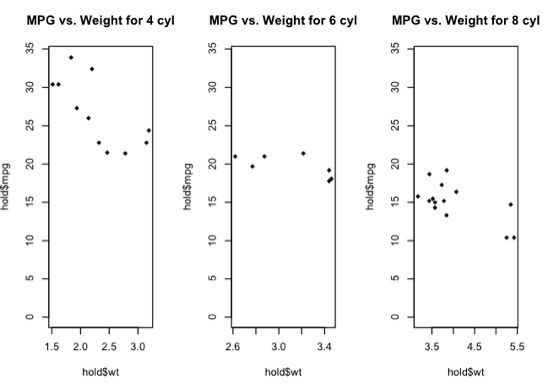
\includegraphics{../IMG/threeplot.png}
\end{center}
\end{frame}

%

\begin{frame}[fragile]
\frametitle{Programming Structures - Using for with matrices}
The for loop structure generalizes to matrices. 
\begin{verbatim}
set.seed(123)
mymat <- matrix(round(rnorm(6),2),3,2)

for (ii in 1:nrow(mymat)) {
  cat("The sum of row",ii,"is",sum(mymat[ii,]),"\n")
}

The sum of row 1 is -0.49 
The sum of row 2 is -0.1 
The sum of row 3 is 3.28 
\end{verbatim}
\end{frame}

%

\subsection{if statement}
\begin{frame}[fragile]
\frametitle{Programming Structures - if}
This is an easy structure. It tests a logical expression, which results in either or a TRUE or FALSE condition, and, based on that, executes a specific block of code 
\small
\begin{verbatim}
if (logical_expression) {
   do something
   ...
}
 
if (logical_expression) {
  do something
  ..
} else {
  do something else
  ...
}
\end{verbatim}
\end{frame}

%

\begin{frame}[fragile]
\frametitle{Programming Structures - if}
Here is a basic example
\small
\begin{verbatim}
( x <- 3)
[1] 3

if (is.numeric(x)) {
   print("x is a number")
} 

[1] "x is a number"

if (x != 3) {
     print("x is not equal to 3")
} else {
    print("guess what ? x is in fact equal to 3")
}
[1] "guess what ? x is in fact equal to 3"
\end{verbatim}
\end{frame}

%

\begin{frame}[fragile]
\frametitle{Programming Structures - if/else}
Here is a more involved if statement that tests for several conditions. It uses the ``else'' keyword in addition to ``if''. Note that an ``if'' statement does not require an ``else'' statement but an ``else'' statement requires a ``parent'' if statement.
\small
\begin{verbatim}
some.num <- 3               

if (some.num < 3) {        # A more involved if statement
     print("Less than 3")
} else if (some.num > 3) {
     print("Greater than 3")
} else {
     print("Must be equal to 3")
}
[1] "Must be equal to 3"
\end{verbatim}
\end{frame}

%

\begin{frame}[fragile]
\frametitle{Programming Structures - if/else}
if/else statements show up a lot in functions. Checking for valid arguments is a common practice.
\small
\begin{verbatim}
x <- 4 
y <- 5

if (!is.numeric(x) | !is.numeric(y)) {
   stop("I need numeric values to do this")
} else {
   if (x == y) {
       print("Equal")
   } else {
      print("Not equal")
   }
}

[1] "Not equal"
\end{verbatim}
\end{frame}


%

\begin{frame}[fragile]
\frametitle{Programming Structures - ifelse}
\begin{itemize}
\item R supports a command called \textbf{ifelse} that is desgined to work specifcally on vectors. 

\item It works well for very large vectors. The format is \textbf{ifelse(test,yes,no)} where
``test'' is a logical expression to be evaluated. 

\item If it is TRUE then the action specified in the ``yes'' position will be executed. If the evaluated expression is FALSE then the action specified in the ``no'' position is executed.
\end{itemize}
\footnotesize
\begin{verbatim}
some.data = rnorm(10000,0,2)
colors = ifelse(some.data < 0,"RED","GREEN")
plot(some.data,col=colors)

# This would be the same as:

for (ii in 1:length(some.data)) {
    if (some.data[ii] < 0) {
       colors[ii] = "RED"
    } else {
       colors[ii] = "GREEN"
    }
}
\end{verbatim}
\end{frame}

%

\begin{frame}[fragile]
\frametitle{Programming Structures - ifelse}
\scriptsize
\begin{verbatim}
some.data <- rnorm(10000,0,2)
colors <- ifelse(some.data < 0,"RED","GREEN")
plot(some.data,col=colors)

# This would be the same as:

for (ii in 1:length(some.data)) {
    if (some.data[ii] < 0) {
       colors[ii] <- "RED"
    } else {
       colors[ii] <- "GREEN"
    }
}
\end{verbatim}
\begin{center}
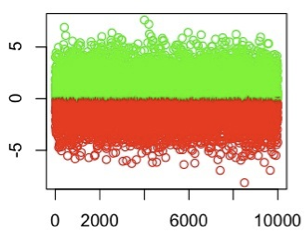
\includegraphics[height=4cm,width=6cm]{../IMG/greenred.png}
\end{center}
\end{frame}

%

\begin{frame}[fragile]
\frametitle{Programming Structures - ifelse}
We can use ifelse when we want to turn some continuous quantity within a data frame into a factor that we can then use to group by
\footnotesize
\begin{verbatim}
mtcars$rating <- ifelse(mtcars$mpg >= mean(mtcars$mpg), "blue", "red")
\end{verbatim}
\scriptsize
\begin{verbatim}
head(mtcars)
                   mpg cyl disp  hp drat    wt  qsec vs am gear carb rating
Mazda RX4         21.0   6  160 110 3.90 2.620 16.46  0  1    4    4   blue
Mazda RX4 Wag     21.0   6  160 110 3.90 2.875 17.02  0  1    4    4   blue
Datsun 710        22.8   4  108  93 3.85 2.320 18.61  1  1    4    1   blue
Hornet 4 Drive    21.4   6  258 110 3.08 3.215 19.44  1  0    3    1   blue
Hornet Sportabout 18.7   8  360 175 3.15 3.440 17.02  0  0    3    2    red
Valiant           18.1   6  225 105 2.76 3.460 20.22  1  0    3    1    red
\end{verbatim}
\footnotesize
\begin{verbatim}
plot(mtcars$mpg~mtcars$wt,col=mtcars$rating,pch=19, main="MPG vs wt")

grid()

legend("topright", c("> mean","< mean"), pch=19,
        col=c("blue","red"),title="Legend",cex=0.7)
\end{verbatim}
\end{frame}
%

\begin{frame}[fragile]
\frametitle{Programming Structures - ifelse}
\begin{center}
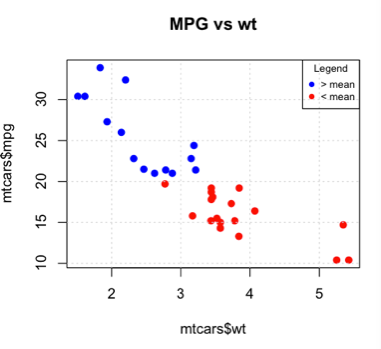
\includegraphics{../IMG/ifelse.png}
\end{center}
\end{frame}

%

\begin{frame}[fragile]
\frametitle{Programming Structures - ifelse}
We can use ifelse when we want to turn some continuous quantity within a data frame into a factor that we can then use to group by
\footnotesize
\begin{verbatim}
mtcars$rating <- ifelse(mtcars$mpg >= mean(mtcars$mpg), "blue", "red")
\end{verbatim}
\scriptsize
\begin{verbatim}
head(mtcars)
                   mpg cyl disp  hp drat    wt  qsec vs am gear carb rating
Mazda RX4         21.0   6  160 110 3.90 2.620 16.46  0  1    4    4   blue
Mazda RX4 Wag     21.0   6  160 110 3.90 2.875 17.02  0  1    4    4   blue
Datsun 710        22.8   4  108  93 3.85 2.320 18.61  1  1    4    1   blue
Hornet 4 Drive    21.4   6  258 110 3.08 3.215 19.44  1  0    3    1   blue
Hornet Sportabout 18.7   8  360 175 3.15 3.440 17.02  0  0    3    2    red
Valiant           18.1   6  225 105 2.76 3.460 20.22  1  0    3    1    red
\end{verbatim}
\footnotesize
\begin{verbatim}
plot(mtcars$mpg~mtcars$wt,col=mtcars$rating,pch=19, main="MPG vs wt")

grid()

legend("topright", c("> mean","< mean"), pch=19,
        col=c("blue","red"),title="Legend",cex=0.7)
\end{verbatim}
\end{frame}
%

\subsection{if and for}
\begin{frame}[fragile]
\frametitle{Programming Structures - if statements and for loops}
\scriptsize
\begin{verbatim}
score <- c(74,68,98,90,100,67,59)   # Exam scores to be graded
for (ii in 1:length(score)) {
  if (score[ii] == 100) {
      grade <- "A+"
  } else if (score[ii] >= 90) {
      grade <- "A"
  } else if (score[ii] >= 80) {
      grade <- "B"
  } else if (score[ii] >= 70) {
      grade <- "C"
  } else if (score[ii] >= 60) {
      grade <- "D"
  }
  else {
    grade <- "F"
  }
  print(grade)
}
[1] "C"
[1] "D"
[1] "A"
[1] "A"
[1] "A+"
[1] "D"
[1] "F"
\end{verbatim}
\end{frame}

%

\begin{frame}[fragile]
\frametitle{Programming Structures - if statements and for loops}
\footnotesize
\begin{verbatim}
set.seed(123)
x <- round(runif(9,1,20))         # Are the elements in x odd or even
[1]  6 16  9 18 19  2 11 18 11

for (ii in 1:length(x)) {
    if (x[ii] %% 2 == 0) {
        print(TRUE)
    }
    else {
        print(FALSE)
    }
}
[1] TRUE
[1] TRUE
[1] FALSE
[1] TRUE
[1] FALSE
[1] TRUE
[1] FALSE
[1] TRUE
[1] FALSE
\end{verbatim}
\end{frame}


%

\begin{frame}[fragile]
\frametitle{Programming Structures - if statements and for loops}
This example mimics the bracket notation 
\footnotesize
\begin{verbatim}
set.seed(123)
x <- round(runif(10,1,20))
[1]  7 13 16  8 13 19  9 11 13 11

logvec <- vector()            # Setup an empty vector
for (ii in 1:length(x)) {
    if (x[ii] %% 2 == 0) {
        logvec[ii] <- TRUE
    }
    else {
        logvec[ii] <- FALSE
    }
}
logvec
[1]  TRUE  TRUE FALSE  TRUE FALSE  TRUE FALSE  TRUE FALSE  TRUE

x[logvec]
[1]  6 16 18  2 18 10
\end{verbatim}
\end{frame}

%

\begin{frame}[fragile]
\frametitle{Programming Structures - if statements and for loops}
One can easily ``break'' out of a for loop based on some condition. Normally you should clean your data before processing but perhaps not 
\newline
\\
Let's say that you are processing elements of a vector and if you encounter a value of NA then you want to stop the for loop
\footnotesize
\begin{verbatim}
my.vec <- c(1,2,3,NA,5,6,7,8,9,10)

for (ii in 1:length(my.vec)) {
    if (is.na(my.vec[ii])) {
       break
    }
    cat("element is ",ii,"\n")
}

element is  1 
element is  2 
element is  3 
\end{verbatim}
\end{frame}

\begin{frame}[fragile]
\frametitle{Programming Structures - if statements and for loops}
Here we want to ``catch'' the the missing value and then ``skip over it''.  To do this we would use the ``next'' statement.
\footnotesize
\begin{verbatim}
my.vec <- c(1,2,3,NA,5,6,7,8,9,10)

for (ii in 1:length(my.vec)) {
    if (is.na(my.vec[ii])) {
       next
    }
    cat("element is ",ii,"\n")
}

element is  2 
element is  3 
element is  5 
element is  6 
element is  7 
element is  8 
element is  9 
element is  10 
\end{verbatim}
\end{frame}

%

\begin{frame}[fragile]
\frametitle{Programming Structures - if statements and for loops}
Here is an example that will be useful when processing things like genetic sequences. Let's say we have a string of text we wish to "encode" by changing all vowels to something else. This would not be a tough code to break but let's see what is involved. In our code we:
\footnotesize
\begin{verbatim}
We'll change          a to s, 
                      e to t, 
                      i to u, 
                      o to v, 
                      u to w 
\end{verbatim}
\normalsize
So a string like:
\footnotesize
\begin{verbatim}

sequence <- "Hello my name is Ed. Happy to meet you" 
\end{verbatim}
\normalsize
would come out like:
\footnotesize
\begin{verbatim}
                 "Htllv my nsmt us td. Hsppy tv mttt yvw"
\end{verbatim}
\end{frame}

%

\begin{frame}[fragile]
\frametitle{Programming Structures - if statements and for loops}
\footnotesize
\begin{verbatim}
sequence <- "Hello my name is Ed. Happy to meet you" 

seq <- unlist(strsplit(sequence,""))

[1] "H" "e" "l" "l" "o" " " "m" "y" " " "n" "a" "m" "e" " " 
    "i" "s" " " "E" "d" "." " " "H" "a" "p" "p" "y" " " "t" 
    "o" " " "m" "e" "e" "t" " " "y" "o" "u"

sequence <- "Hello my name is Ed. Happy to meet you" 

seq < unlist(strsplit(sequence,""))
for (ii in 1:length(seq)) {

  # Write code to inspect each element of seq to determine if it is 
  # a candidate for changing.

}

"Htllv my nsmt us Ed. Hsppy tv mttt yvw"

\end{verbatim}
\end{frame}

%

\subsection{while statement}
\begin{frame}[fragile]
\frametitle{Programming Structures - while}
The \textbf{while} loop is similar to the for loop. We have some expression that must be evaluated until some condition is met. This is useful when we are writing code that must converge on something.  
\footnotesize
\begin{verbatim}
sum <- 0 
n <- 1000
i <- 1
while (i <= n) {
    sum <- sum + i
    i <- i + 1
}
sum
[1] 500500
#   The following is equivalent
sum <- 0
n <- 1000
for (i in 1:n) {
   sum <- sum + 1
}
sum
\end{verbatim}
\end{frame}


%

\begin{frame}[fragile]
\frametitle{Programming Structures - while }
Taking the square root of a number and then taking the square root of that result and so will
eventually converge to 1. We can use a while loop to do this
\footnotesize
\begin{verbatim}
num <- 13
sqrtval <- sqrt(num)

# Loop until the sqrt value becomes equal to 1

while ( sqrtval != 1)  {    
  sqrtval <- sqrt(sqrtval)

# sprintf allows us to format a variable according to a pattern
# See http://www.cookbook-r.com/Strings/Creating_strings_from_variables/

  print(sprintf("%2.12f",sqrtval))
}
\end{verbatim}
\end{frame}


%
\begin{comment}
\begin{frame}[fragile]
\frametitle{Programming Structures - while - \alert{Supplemental}}
This example drives home how a \textbf{while loop} can be useful. We will implement Newton's method to find the square root of a number 
\begin{itemize}
\item First we make a guess, square it and see how close we came 
\item If the difference between our guess squared and the target number is less than a specified amount then we are done. 
\item But while this is \textbf{not} TRUE then we keep guessing using Newton's help
\end{itemize}
\footnotesize
\begin{verbatim}
N <- 121     # The number whose square root we wish to estimate
guess <- 9   # Our first guess (its not so good but we can improve it)

abs(N - (guess^2))
[1] 40                # Wow. Our first guess isn't so good.

\end{verbatim}
\end{frame}

%

\begin{frame}[fragile]
\frametitle{Programming Structures - while - \alert{Supplemental}}
Newton comes to the rescue by giving us a formula to improve the guess. We take our target number, divide it by the guess, and add the resulting ratio to the value of the guess. We then multiply this result by 0.5 
\footnotesize
\begin{verbatim}
guess <- 0.5*(N/guess + guess)
[1] 11.22222                   # Better but not quite there yet

abs(N - (guess^2))
[1] 4.933284

guess = 0.5*(N/guess + guess)  # Even better
abs(N - (guess^2))
[1] 0.04840968

guess = 0.5*(N/guess + guess)  # Perfect.
abs(N - (guess^2))
[1] 4.84e-06

guess
[1] 11
\end{verbatim}
\end{frame}

%

\begin{frame}[fragile]
\frametitle{Programming Structures - while - \alert{Supplemental}}
Implementing Newton's method to find the square root of a number if easy with a while loop
\footnotesize
\begin{verbatim}
n <- 121

iterations <- 1

guess <- 9

tolerance <- 0.0001

diff <- n-(guess^2)

while (abs(diff) >= 0.001) {
    cat("Iteration number ",iterations,"\n")
    guess <- (n/guess + guess)/2
    diff <- n-(guess^2)
    iterations <- iterations + 1
}
Iteration number  1 
Iteration number  2 
Iteration number  3 

guess
[1] 11
\end{verbatim}
\end{frame}

\end{comment}
%%% End of document
\end{document}
